\chapter{最新の脆弱性}

本章では、今年度に発生した重大な脆弱性について、その概要と脆弱性の内容、および対策手段をまとめる。
Heartbleed脆弱性、Shellshock脆弱性、POODLE脆弱性を紹介する。

\section{Heartbleed}

\subsection{概要}
ハートブリード(CVE-2014-0160)\cite{cve}とは,2014年4月に発覚したオープンソース暗号化ライブラリ「OpenSSL」のソフトウェア・バグのことで
ある.発表によると,認証局から認定を受けた「安全な」インターネット・Webサーバの約17%(約50万台)\cite{wiki}に脆弱性があり,
サーバの秘密鍵や利用者のセッション・クッキーやパスワードを盗み出すことが出来る状態にあった.
この脆弱性は,OpenSSL バージョン1.0.1/1.0.2系に存在し,Heartbeat拡張の実装に見つかった致命的なバグであることから,
``Heartbleed''バグと称されている.

\subsubsection{発覚の経緯}
\begin{itemize}
\item 2011年12月31日 : ロビン・シーゲルマンがgitにパッチを提出し,OpenSSLの開発チームがレビュー
\item 2012年 3月14日 : 脆弱性が混入したコードはOpenSSL バージョン1.0.1に採用され,が公開
\item 2014年 3月21日 : グーグルのボド・モエラーとアダム・ラングレーがレッドハットのバグ管理システムに修整プログラムを登録
\item 2014年 3月31日 : CloudFlare社が自社製品を修整
\item 2014年 4月01日 : Googleのセキュリティーチームのニール・メータ2012年3月14日以降のOpenSSL 1.0.1シリーズの全ての版にバグあると発表
\item 2014年 4月03日 : コデノミコン社がNCSC-FIにハートブリード・バグを報告
  \begin{itemize}
  \item 独自に新しく開発中だった暗号化・認証プロセスのテストツール検証の過程で発見\cite{hb}.
  \end{itemize}

\item 2014年 4月07日 : OpenSSLがバグを修整したOpenSSL 1.0.1gを公開
\item 2014年 4月24日 : Linux Foundationが大手IT企業と共に「Core Infrastructure Initiative」を設立し,OpenSSLに援助
\end{itemize}

しかし,数人の攻撃者は問題発覚の少なくとも5ヶ月前に欠陥を発見していたことが監査ログから分かっている\cite{ars}\cite{erratasecurity}.


\subsection{脆弱性の内容}
HeartbleedとはOpenSSL の Heartbeat Extension という機能の脆弱性である.
OpenSSL ではこの実装に意図しないメモリ領域のデータを返してしまう という致命的なバグが存在した.
Heartbeat Extensionでは,返却するパケットを生成する際に,受け取ったパケットをメモリ上に保持し,
その先頭から"データ長"の分だけメモリのデータをコピーして返却しているが,
問題のOpenSSL の実装では,この"データ長"と実際のパケットの長さを境界検査をせずに,
受け取った"データ長"をそのまま利用しているため,
実際のデータの長さよりも大きな値を設定されるとHeartbeatパケットのデータだけでなく,
本来関係のないメモリ上のデータまでコピーされてしまうというものである.


\subsubsection{Heartbeat Extension}
"Heartbeat Extension" というプロトコルが RFC6520\cite{rfc6520}で定義されている.
RFCによると,``HeartbeatRequest''は``HeartbeatResponse''のメッセージが返される必要があるとしている.
具体的なHeartbeat Extension の通信の中身は Heartbeat のパケットが送られてきたらその内容をコピーし,
ヘッダのtypeを"Heartbeatレスポンス"に書き換えて返却するという仕様である.
TLSでは keep-aliveのようにセッションの再構築を避け,
SSLのセッションをより長く保持することができるものである.
また,DTLS では MTU のサイズをテストするための probeパケットとして利用している.


\subsubsection{問題部分のコード}
\subsubsubsection{ssl\/d1\_both.c dtls1\_process\_heartbeat()}
\begin{verbatim}
// p: パケットのデータを保持したメモリのポインタ
unsigned char *p = &s->s3->rrec.data[0], *pl;
unsigned short hbtype;
unsigned int payload;
unsigned int padding = 16; /* Use minimum padding */

hbtype = *p++;
// ここでpayloadに"データ長"の値がセットされる
n2s(p, payload);
pl = p;

~~~~~(省略)~~~~

// メモリ領域の確保(type用の1byte,length用の2byte
// そして実データの長さpayloadで設定された大きさ に余白(これは16byteに設定されている)を合わせて大きさを確保)
buffer = OPENSSL_malloc(1 + 2 + payload + padding);
bp = buffer;

~~~~~(省略)~~~~

// typeに"Heartbeatレスポンス"を設定する
*bp++ = TLS1_HB_RESPONSE;  // 先頭1byteにheart beatのtypeを設定
s2n(payload, bp);          // payloadに設定されている値をbpの次の2byteに設定

// 応答パケットをメモリ上に作成
memcpy(bp, pl, payload);
/* ユーザからのリクエストから得たpayload分の長さのデータをplからbpにコピー
 * 実際のplに入っているデータ長がpayloadに設定されている値よりも短い場合,
   plから連続したメモリ領域をbpに コピーしてしまう*/
\end{verbatim}

\subsubsubsection{pの構造体}
\begin{verbatim}
/* dataが実際に受け取っているデータ.このデータは先頭1byteがheart beatのtypeを表し,
   次の2byteがそのリクエストの長さを表すような データになっている.*/
typedef struct ssl3_record_st
    {
        int type;               /* type of record */
        unsigned int length;    /* How many bytes available */
        unsigned int off;       /* read/write offset into 'buf' */
        unsigned char *data;    /* pointer to the record data */
        unsigned char *input;   /* where the decode bytes are */
        unsigned char *comp;    /* only used with decompression - malloc()ed */
        unsigned long epoch;    /* epoch number, needed by DTLS1 */
        unsigned char seq_num[8]; /* sequence number, needed by DTLS1 */
    } SSL3_RECORD;
\end{verbatim}

\subsubsubsection{マクロ}
\begin{verbatim}
/* straight from the openssl source */
#define n2s(c,s)    ((s=(((unsigned int)(c[0]))<< 8)| (((unsigned int)(c[1])) )),c+=2)
#define s2n(s,c)    ((c[0]=(unsigned char)(((s)>> 8)&0xff), c[1]=(unsigned char)
(((s) )&0xff)),c+=2)
\end{verbatim}

\subsubsection{観測結果}
NICTのサイバーセキュリティ情報遠隔分析基盤NONSTOPを用いて,Darknetに関するトラフィックデータを分析した.
その結果.この脆弱性が4月に公表されたことに着目し,httpsのポートスキャンを行なったipアドレスの数を集計したところ,図\ref{fig:https}のように4月中旬から
その数が増加していることがわかった.

\begin{figure}[htbp]
  \centering
    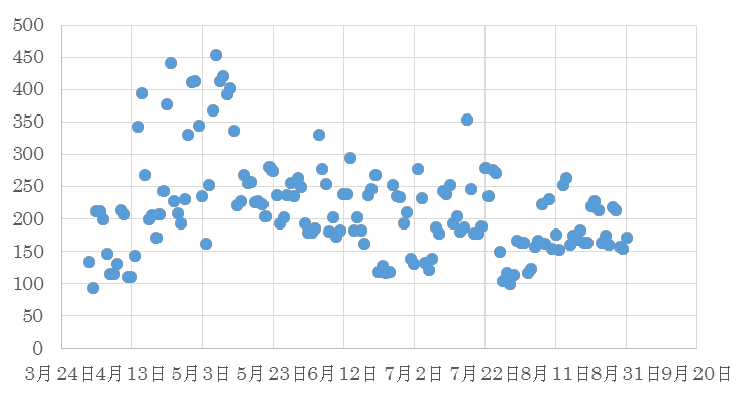
\includegraphics[scale=0.38]{https.png}
    \caption{Darknetの観測結果}
  \label{fig:https}
\end{figure}


\subsection{対策}
\subsubsection{脆弱性の検知}
\begin{itemize}
\item SSLチェックツール(\url{https://sslcheck.globalsign.com/ja})\cite{check}などを用いて,判定する.
\item ターミナル上で「openssl version -a」と実行し,バージョンが 1.0.1 〜 1.0.1fまでの間なら,脆弱性が存在すると判定する.
\end{itemize}


\subsubsection{対策}
対策としては以下のような対策が考えられる.
\begin{itemize}
\item 脆弱性を修正したバージョン(1.0.1g以降)への更新する.
\item オプションで\verb|DOPENSSL_NO_HEARTBEATS|を付けて再コンパイルする.
\item IDS/IPSを用いる.
\end{itemize}

\section{Shellshock}

\subsection{概要}

Shellshockは,bash (Bourne-Again SHell)
というシェルにおける一連の脆弱性の名称である.\cite{uscert}
この脆弱性が存在するシステムにおいては,攻撃者が任意のコマンドを実行できてしまう.bashは
多くのUNIXベースの環境においてデフォルトのシェルとして使用されているため,非常に広範囲に
渡って影響を与える脆弱性である.また,bashを用いて間接的にコマンドを実行するプログラム
(例:Apacheのmod\_cgi・OpenSSHのsshd・DHCPクライアント・qmailなど)
も影響を受けるため,攻撃者はリモート環境から攻撃することも可能になる.

\subsection{脆弱性の内容}

Shellsock脆弱性の原因は,bashの環境変数の処理におけるバグである.\cite{cve20146271}
bashの機能の1つとして,よく使う処理を関数として定義し,後ほど再利用する機能がある.

\begin{verbatim}
function hello {
 echo "Hello, world!"
}
hello
\end{verbatim}

上記のコードでは\texttt{hello}という関数を定義し,次に呼び出している.また,bashでは環境
変数を用いて定義することもできる.

\begin{verbatim}
env hello="() { echo 'Hello, world!'; }" bash -c hello
\end{verbatim}

上記のコードのように,\texttt{() \{}で始まる文字列を環境変数に設定すると,新しく開いたシェル
で関数定義が暗黙的にインポートされ,使用できるようになる.この挙動もbashの仕様の範囲
内である.Shellshock脆弱性の原因となったのは,このような環境変数での関数定義の
後ろに続くコードまで実行してしまっていたことである.

\begin{verbatim}
env x="() { :;}; echo 'vulnerable'" bash -c "echo this is a test"
\end{verbatim}

上記の例では環境変数\texttt{x}に空の関数定義を設定しているが,その際に関数定義の後ろの
\texttt{echo "vulnerable"}まで実行してしまう問題があった.シェルを開くたびに関数定義
の後ろのコードが実行されるため,攻撃者はこれを利用することで,任意のコードを実行
できてしまう.
他にもbashのパーサには様々なバグが存在し,これらを利用することで任意のコードの実行や
DoS攻撃が可能になってしまっていた.\cite{cve20147169, cve20147186, cve20147187, cve20146277, cve20146278}

また,間接的にbashを実行しているアプリケーションもこの脆弱性の対象となった.例えば,
Apacheで動的コンテンツを配信するためのモジュールであるmod\_cgiは,WebサーバからCGI
スクリプトに対してデータを渡すために,シェルの環境変数を利用していた.よって,クライアント
から悪意のあるHTTPリクエストを送信することで,Shellshock脆弱性をつくことができる.

\begin{verbatim}
GET / HTTP/1.1
User-Agent: () { :;}; echo vulnerable
\end{verbatim}

上記の例では,\texttt{User-Agent}に攻撃コードが設定されている.mod\_cgiでは\texttt{User-Agent}の
値は環境変数に設定されるので,その際に\texttt{echo vulnerable}が実行されてしまう.
同様の攻撃がOpenSSHのsshd,DHCPクライアント,qmailなどについても可能である.

\subsection{対策}

Shellshock脆弱性に対する最も直接的かつ効果的な対策は,bashのアップデートである.脆弱性を
防ぐパッチを当てたバージョンのbashが配布されているので,これで利用しているbashの
バイナリを置き換えることによって対策を行える.また,主要なLinuxディストリビューション
からはパッチしたbashをインストールするパッケージが提供されているので,より簡単に
脆弱性対策が可能である.関数自動インポート機能自体がセキュリティリスクであるとし,
デフォルトではbashの関数自動インポート機能を無効にしているディストリビューションもある.\cite{freebsd}
